\documentclass[../ZF_HM2.tex]{subfiles}

\begin{document}

\begin{itemize}
	\item \textcolor{magenta}{Summierte Rechteckregel ist genauer als die summierte Trapezregel}
	\item \textcolor{magenta}{Summierte Simpsonregel ist am genaustren(verglichen mit sum.Recht.und Trap.)}
	\item \textcolor{magenta}{Faktor Fehlerabschätzung summ.Rechteckregel $<$ summ.Trap.Regel = 2}

\end{itemize}

\subsection{Rechteck- und Trapezregel}
Annäherung bestimmtes Integral.\\
\textbf{Rechtecksregel / Mittelpunktsregel:\\}
\colorbox{orange!30}{$Rf = f(\dfrac{a+b}{2})*(b-a)$}\\
\colorbox{pink!30}{$Tf = \dfrac{f(a)+f(b)}{2}*(b-a)$}
\subsubsection{Summierte Rechkteckregle / summierte Trapezregel}
\colorbox{yellow!30}{h=}$\dfrac{b-a}{n}$; \colorbox{green!30}{$x_i$}$= a+i*$ \colorbox{yellow!30}{h}; $x_n=b$; (i=0,...,n-1)\\
\colorbox{orange!30}{$Rf(h)=h*\sum_{i=0}^{n-1}f(x_i+\dfrac{h}{2})$}\\
\colorbox{pink!30}{$Tf(h)=h*(\dfrac{f(a)+f(b)}{2}+\sum_{i=1}^{n-1}f(x_i))$}\\
n = Anzahl Subintervalle [$x_i,x_{i+1}$]\\
\subsection{Simpsonregel}
\colorbox{orange!30}{$Sf=\dfrac{(b-a)}{6}(f(a)+4f(\dfrac{a+b}{2})+f(b))$}

\subsubsection{Summierte Simpsonregel}
\colorbox{orange!30}{$Sf(h)=\dfrac{h}{3}(\dfrac{1}{2}f(a)+\sum_{i=1}^{n-1}f(x_i)+2\sum_{i=1}^{n}f(\dfrac{x_{i-1+x_i}}{2})+\dfrac{1}{2}f(b))$}
\subsection{Fehler der summierten Quadraturformeln}
$|\int_a^bf(x)dx-Rf(h)|\leq \dfrac{h^2}{24}(b-a)*max|f''(x)|$\\
$|\int_a^bf(x)dx-Tf(h)|\leq \dfrac{h^2}{12}(b-a)*max|f''(x)|$\\
$|\int_a^bf(x)dx-Sf(h)|\leq \dfrac{h^4}{2880}(b-a)*max|f^{(4)}(x)|$\\
Schritte berechnen bis Tol. erreicht:

$\dfrac{h^2}{24}(b-a)\leq Tol$      $|*\dfrac{24}{(b-a)} $etc...(Analog für andere Formel)\\

\subsection{Gauss-Formeln}
$x_i$ Stützstellen müssen nicht äquidistant sein $\implies$ so wählen, dass $\int_a^bf(x)dx$ optimal approximiert. $a_i,x_i$ so wählen, dass Fehlerordnung möglichst hoch bzw. Fehler möglichst klein.
\begin{mdframed}
	\textbf{Gauss-Formeln für \colorbox{blue!30}{n=1,2,3: $\int_a^bf(x)dx\sim \dfrac{b-a}{2}\sum_{i=1}^{n}a_i f(x_i)$}}\\
	\colorbox{violet!30}{n=1: $G_1f =$}$(b-a)*f(\dfrac{b+a}{2})$\\
	\colorbox{green!30}{n=2: $G_2f =$}$\dfrac{b-a}{2}[f(-\dfrac{1}{\sqrt{3}}*\dfrac{b-a}{2}+ \dfrac{b+a}{2})]$\\
	\colorbox{orange!30}{n=3: $G32f =$}$\dfrac{b-a}{2}[\dfrac{5}{9}*f(-\sqrt{0.6}*\dfrac{b-a}{2}+\dfrac{b+a}{2})+\dfrac{3}{9}*f(\dfrac{b+a}{2})]+\dfrac{b-a}{2}[\dfrac{5}{9}*f(-\sqrt{0.6}*\dfrac{b-a}{2}+\dfrac{b+a}{2})]$

\end{mdframed}

\subsection{Romberg-Extrapolation}

\colorbox{orange!30}{$T_{j0}=$}$Tf(\underbrace{\dfrac{b-a}{2^j}}_\text{(=h)})$, Für j=0,1,...,m-k\\\\
\colorbox{orange!30}{$T_{jk}=$}$\dfrac{4^k*T_{j+1,k-1}-T_{j,k-1}}{4^k-1}$, Für k=1,2,...,m und j=0,1,...,m-k\\\\
= Näherungen der Fehlerordnung \colorbox{green!30}{$2k+2$} gegeben.\\
\colorbox{blue!30}{Romberg-Folge:} \colorbox{orange!30}{$h_j$=}$\dfrac{b-a}{2}$\\
$n_j=2^j$, $x_i= a+ih_j$\\
\begin{figure}[H]
\centering
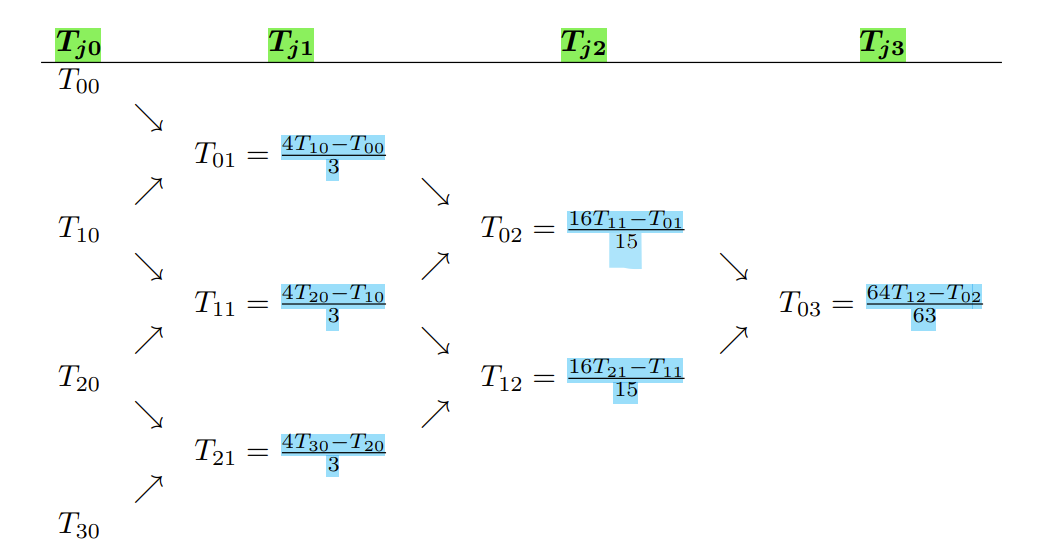
\includegraphics[width=0.3\textwidth]{Resources/Images/RombergExtrapolation.png}
\caption{\label{fig:RombergExtrapolation}RombergExtrapolation.}
\end{figure}
































\end{document}